\documentclass{article}

\usepackage[utf8]{inputenc}
\usepackage{ctex}
\usepackage{assignpkg}
\usepackage{xeCJK}
\usepackage{amsmath, amsthm, amssymb}
\usepackage{listings,xcolor}
\usepackage{geometry} % 设置页边距
\usepackage{fontspec}
\usepackage{graphicx}
\usepackage[colorlinks]{hyperref}
\usepackage{setspace}
\usepackage{fancyhdr} % 自定义页眉页脚
\usepackage{enumerate}
\usepackage{ulem}
\usepackage{scalerel}
\usepackage{stackengine}
\usepackage{xcolor}
\usepackage{polynom}
\usepackage{algorithm}
% \usepackage{algorithmic}
\usepackage{algpseudocode}
\usepackage{chngcntr}
\usepackage{smartdiagram}
\newcommand\showdiv[1]{\overline{\smash{\hstretch{.5}{)}\mkern-3.2mu\hstretch{.5}{)}}#1}}
\newcommand\ph[1]{\textcolor{white}{#1}}

\counterwithin{figure}{subsection}
\counterwithin{table}{subsection}

\newtheorem*{thmm}{定理}
\newtheorem{thm}{定理}[section]
\newtheorem{definition}{定义}[section]
\newtheorem{lemma}{引理}[section]
\newtheorem{corollary}{推论}[section]
\newtheorem{prop}{命题}[section]
\newtheorem{attr}{性质}[section]
\newtheorem*{prf}{证明}
\newtheorem*{lprf}{引理证明}
\newtheorem{exm}{例}[section]
\newtheorem*{sol}{解}


\linespread{1.2}

\definecolor{dkgreen}{rgb}{0,0.6,0}
\definecolor{gray}{rgb}{0.5,0.5,0.5}
\definecolor{mauve}{rgb}{0.58,0,0.82}

\pagestyle{fancy}

\lhead{\CJKfamily{kai} Xi'an JiaoTong University} %以下分别为左中右的页眉和页脚
\chead{}

\rhead{\CJKfamily{kai} 第 \thepage 页}
\lfoot{} 
\cfoot{\thepage}
\rfoot{}
\renewcommand{\headrulewidth}{0.4pt} 
\renewcommand{\footrulewidth}{0.4pt}
%\geometry{left=2.5cm,right=3cm,top=2.5cm,bottom=2.5cm} % 页边距
\geometry{left=3.18cm,right=3.18cm,top=2.54cm,bottom=2.54cm}
\setlength{\columnsep}{30pt}

\renewcommand{\algorithmicrequire}{ \textbf{Input:}} %Use Input in the format of Algorithm
\renewcommand{\algorithmicensure}{ \textbf{Output:}} %UseOutput in the format of Algorithm

\makeatletter

\makeatother

\lstset{
    language    = c++,
    numbers     = left,
    numberstyle={                               % 设置行号格式
        \small
        \color{black}
        % \fontspec{Consolas}
    },
	commentstyle = \color[RGB]{0,128,0}\bfseries, %代码注释的颜色
	keywordstyle={                              % 设置关键字格式
        \color[RGB]{40,40,255}
        % \fontspec{Consolas Bold}
        \bfseries
    },
	stringstyle={                               % 设置字符串格式
        \color[RGB]{128,0,0}
        % \fontspec{Consolas}
        \bfseries
    },
	basicstyle={                                % 设置代码格式
        % \fontspec{Consolas}
        \small\ttfamily
    },
	emphstyle=\color[RGB]{112,64,160},          % 设置强调字格式
    breaklines=true,                            % 设置自动换行
    tabsize     = 4,
    frame       = single,%主题
    columns     = fullflexible,
    rulesepcolor = \color{red!20!green!20!blue!20}, %设置边框的颜色
    showstringspaces = false, %不显示代码字符串中间的空格标记
	escapeinside={\%*}{*)},
}


% \studentIds{计试91 施劲松}{2193512032}
% \studentNames{姓名}{学号}

\assignmentName{复杂网络动力学基础}
\assignmentNumber{2}
\subTitle{}

\date{10/23/2022}

\begin{document}

\makecover

\section{问题 1}

\subsection{问题描述}

试求 ER 随机网络 $G_{N, p}$ 在 $N=3000$,并在:
\begin{enumerate}
    \item $c=0.5,z=1.0$
    \item $c=1.0,z=1.0$
    \item $c=1.0,z=1.5$
    \item $c=10,z=1.0$
\end{enumerate}
四种情况下的谱密度图,给出实验过程、结果及相关分析。

\subsection{实验原理}

随机网络是由一些节点通过随机连接而组成的一种复杂网络。其构成有两种等价方法:
\begin{enumerate}
    \item ER 模型
    \item 二项式模型
\end{enumerate}
其中 ER 模型为给定 $N$ 个节点,最多可存在 $N(N-1)/2$ 条边,从这些边中随机选择 $M$ 条边就可以得到一个随机网络,它一共可以产生 $C_{N(N-1)/2}^{M}$ 种可能的随机网络,且产生每种随机网络的概率均相同。

随机网络中节点的度分布是遵循 Possion 分布的,有平均度满足:
$$
<k>=p(N-1)\approx pN \quad (N\to\infty)
$$
准确来说,对于某个节点 $v_i$,其度分布 $K$ 满足二项分布,即:
$$
K\thicksim B(N-1,p)
$$

网络频谱是其邻接矩阵 $\mathrm{A}$ 的特征值的集合。一个有 $N$ 个节点的网络必有 $N$ 个特征值 $\lambda_j$,从而定义其谱密度为:
$$
\rho(\lambda)=\frac{1}{N}\sum_{j=1}^{N}\delta(\lambda -\lambda_j)
$$
其中,
$$
\delta(x)=
\begin{cases}
    +\infty,x=0\\
    0,x\neq 0
\end{cases},
\int_{-\infty}^{+\infty}\delta(x){\mathrm{d}}x=1
$$

而对于连接概率为 $p(N)=cN^{-z}$ 的随机网络 $G_{N, p}$ 的特征谱,其平均度为 $<k>=Np=cN^{1-z}$。当 $0\leq z<1$ 时,随机网络中将出现无限聚类体,且当 $N\to\infty$ 时,$<k>\to\infty$。此时,随机网络的频谱密度呈现半圆形分布,并有:
$$
\rho(\lambda)=
\begin{cases}
    \frac{\sqrt{4Np(1-p)-\lambda^2}}{2\pi Np(1-p)},\vert \lambda\vert<2\sqrt{Np(1-p)}\\
    0, otherwise
\end{cases}
$$

\subsection{求解过程}

利用 \lstinline{python} 随机生成 ER 网络进行采样,而后获取邻接矩阵的特征值,计算谱密度。由于采用 Monte-Carlo 的随机采样,为了使不用的采样具有可加性,将谱密度绘成直方图,使得每个特征值都能落向唯一一个区间,方便统计绘图。循环采样,其流程图表示如下:

\begin{center}
    \smartdiagram[circular diagram:clockwise]{设置参数,
        多次采样生成随机ER网络, 获取随机图的谱密度, 统计绘图}
\end{center}

\subsection{实验结果与分析}

实验得到的结果图 \ref{fig:task1}。可以看到:
\begin{itemize}
    \item 当 $z>1$ 时,谱密度图度偏离半圆形结构,这是由于当 $N\to\infty$ 时,$<k>\to 0$,此时 $\rho(\lambda)$ 的奇数阶矩 ${\mathrm{M}}_{p}=0$,这意味着要回到原始节点的路径只能是沿着来时的相同节点返回,网络具有树状结构;
    \item 当 $z=1,c\leq 1$ 时,图像仍不为半圆形,这是因为当 $N\to\infty$ 时,节点平均度 $<k>\approx c$,且 $c\leq 1$,那么网络基本也为树状结构;
    \item 当 $z<1,c>1$ 时,谱密度的奇数矩 ${\mathrm{M}}_{p} \gg 0$,网络结构则发生了显著变化,出现``环''与``分支'',几乎任何结点都属于无限聚类体,谱密度呈现半圆形分布。
\end{itemize}

\begin{figure}[ht]
    \label{fig:task1}
    \centering 
    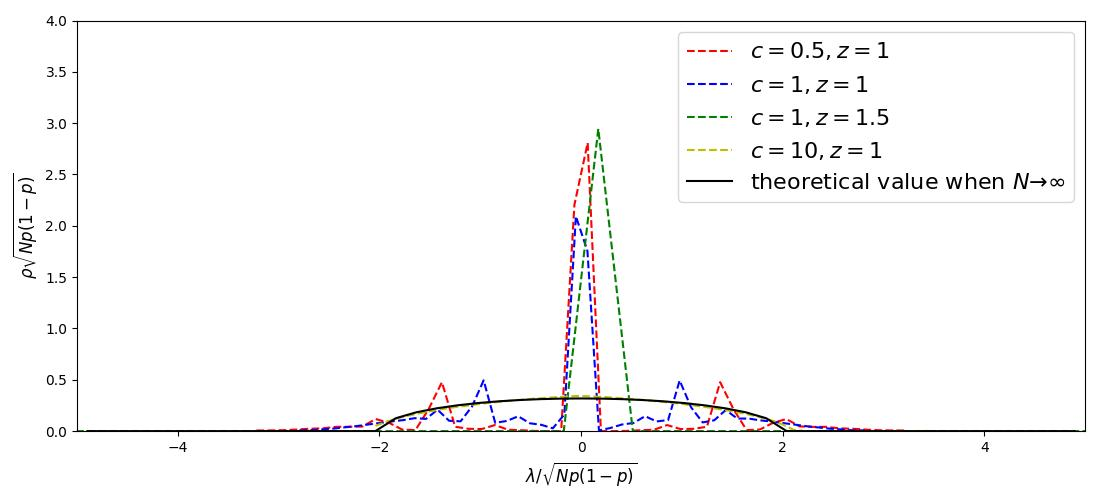
\includegraphics[width=.7\textwidth]{../task1.jpg}
    \caption{问题 1:谱密度图}
\end{figure}

本实验还绘出了 $z<1,c>1,N\to\infty$ 时的谱密度理论分布曲线($\rho'=\frac{\sqrt{4-\lambda'^2}}{2\pi}(\rho'=\sqrt{Np(1-p)\rho}, \lambda'=\lambda/\sqrt{Np(1-p)})$,即图 \ref{fig:task1} 中黑色曲线)可见其与 $z=1.5,c=10$ 图像(图 \ref{fig:task1} 中黄色曲线)基本重合,验证了分析的正确性。

\section{问题 2}

\subsection{问题描述}

试绘制WS小世界网络的度分布 $P(k)$ 图。初始网络为规则网络,选取最近邻耦合网络,其中,节点总数$N=1000$,耦合数$K=6$,$n$为未重连的边数,$\widetilde{n}$ 为重连的边数,随机化重连概率分别为 $p=0,0.1,0.2,0.4,0.6,0.9,1.0$。理论近似计算公式如下:
$$
P(k)\approx \sum_{n=0}^{\min\{k-K/2,K/2\}}C_{K/2}^{n}(1-p)^{n}p^{K/2-n}\frac{(pK/2)^{k-K/2-n}}{(k-K/2-n)!}e^{-pK/2}
$$

试分析度分布公式$P(k)$, 它的未重连边数 $n$ 的求和区间如果选取 $\max(k-K,\frac{K}{2})$,
结果又如何?当 $k\geq K/2$ 时,$k$ 最大值可为多少?请给出实验过程、结果及相关分
析。要求每个节点的度值 $k\geq K/2$ 且保证节点的连通性不被破坏。

\subsection{实验原理}

小世界的概念,简单地说就是用来描述这样一个事实:尽管一些网络系统具有很大的尺寸,但其中任意两个节点之间却有一个相对较小的距离。小世界模型是介于规则网络和随机网络之间的网络。WS 小世界模型基于两个人(Watts 和 Strogatz)的假设,模型从一个完全的规则网络出发,以一定的概率将网络中的连接打乱重连。具体的构造方法如下:
\begin{enumerate}
    \item 构造规则图。例如考虑一个含有 $N$ 个节点的最近邻耦合网络,它们围成一个环,其中每个节点都与它左右两侧的各 $K/2$ 个节点相连,耦合数 $K$ 是偶数;
    \item 随机化重连。将上面规则图中的每条边以概率 $p$ 随机地重新连接,即:将边的一个端点保持不变,而另一个端点以概 $p$ 与网络的其余 $(N-K-1)$ 个节点随机连接。其中规定:任意两个不同的节点之间至多只能有一条边(无重边)。
\end{enumerate}
最后得到的网络称为WS模型网络。

度分布公式如下:
\begin{align}
    P(k) = \sum_{n=0}^{\min(k-K/2,K/2)} C_{K/2}^{n} \binom{k-K/2-n}{k/2} p^{k-2n}
    (1-p)^{K+2n-k}
\end{align}

注意到当$N\to\infty$时,可以用泊松分布近似:
\begin{align}
    P(k) = \sum_{n=0}^{\min(k-K/2,K/2)} C_{K/2}^{n} (1-p)^n p^{K/2-n} \frac{{(pK/2)}^{k-K/2-n}}{(k-K/2-n)!} e^{-pK/2}
    \label{sg}
\end{align}

\subsection{求解过程}

本实验使用随机采样的方式完成,并用度分布公式进行验证。循环采样,流程图如下:
\begin{center}
    \smartdiagram[circular diagram:clockwise]{设置参数,
        多次采样生成随机WS网络, 获取随机图的度分布, 利用泊松分布近似公式计算理论值, 统计绘图}
\end{center}

\subsection{实验结果与分析}

实验结果为图 \ref{fig:task2}。与实验指导书给出的几乎相同。另外图中对应颜色的 $\triangle$ 为利用公式计算的结果,可以发现与随机模拟得到的曲线几乎无异,这就验证了实验及公式的正确性。
\begin{figure}[ht]
    \label{fig:task2}
    \centering
    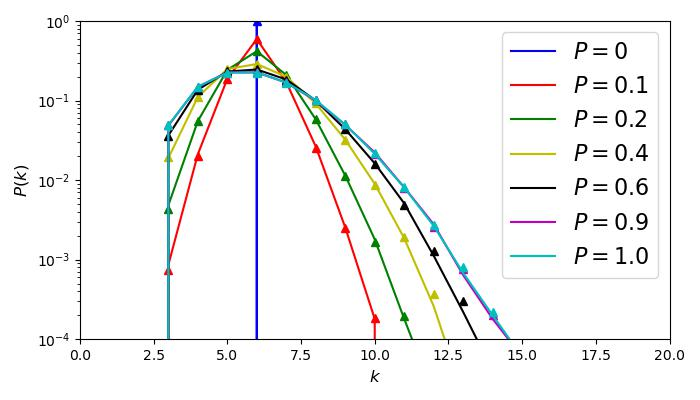
\includegraphics[width=.7\textwidth]{../task2.jpg}
    \caption{问题 2:WS 模型度分布图}
\end{figure}

思考题:
\begin{enumerate}
    \item 它的未重连边数 $n$ 的求和区间如果选取 $\max(k-K,\frac{K}{2})$,结果又如何?\\
    在代码中调整参数绘制图 \ref{fig:task2_fake},可见只有在 $k<K/2$ 时有变化,这是因为当 $k<K/2$ 时,$P(k)$ 计算时只有 $n=0$ 时有贡献,所以在 $k<K/2$ 有值。而注意到当 $n>K/2$ 时 $C_{K/2}^{n}=0$,所以当 $n>K/2$ 无贡献,同理在 $n>k-K/2$ 时亦无贡献,故:$n\leq\min\{k-K/2,K/2\}$,更改上界并无意义。
    \begin{figure}[ht]
        \label{fig:task2_fake}
        \centering
        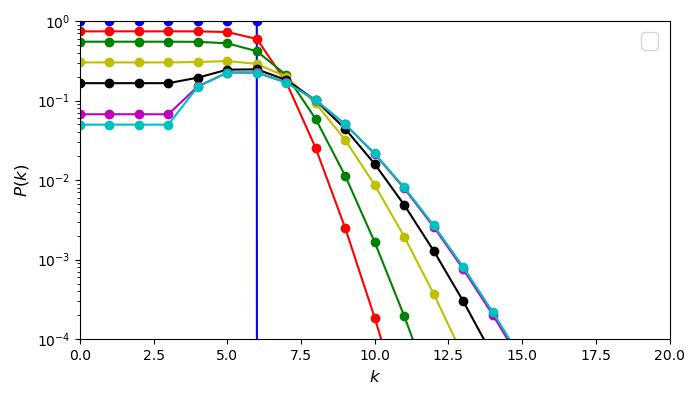
\includegraphics[width=0.7\textwidth]{../task2_fake.jpg}
        \caption{思考题 1:调整上界重绘度分布}
    \end{figure}
    \item 当 $k\geq K/2$ 时,$k$ 最大值可为多少?\\
    答:为 $N-1$,不过此发生的概率极小。
\end{enumerate}

\newpage

\section{感想与建议}

感想:复杂网络动力学对学科研究的意义重大,通过本次实验,我更进一步地理解了复杂网络动力学的内涵,提升自我能力。对经典的复杂网络模型有了一定的了解,并知道如何生成分析 ER 随机网络与 WS 小世界网络,收获颇丰。

建议:第一个问题需要求解矩阵的特征值,而求特征值的算法由于需要计算特征多项式故在求解是会耗费大量时间,可以将 $N$ 的值改小些。

\section{源码}

问题 1 见:\lstinline{./src/task_1.py}。

问题 2 见:\lstinline{./src/task_2.py}。

\section{运行}

请确保安装了 \lstinline{python3} 以及依赖包 \lstinline{numpy}(可使用 conda 或 pip 安装),conda 安装命令并运行方法:
\begin{lstlisting}
$ cd src/
$ conda create -n lab1
$ conda activate lab1
$ conda install --yes --file requirements.txt
$ python3 task.py
\end{lstlisting}

另外,源码采用 utf-8 编码,若开启编辑器中文乱码,请切换至 utf-8 编码重新打开。

\end{document}